\subsection{Multi-Model Comparison}
\label{subsec:multi-model}

To assess whether the annotation findings are specific to Claude Sonnet or generalisable across large language models, the same prompt and classification schema were applied using OpenAI GPT-4o-mini. Table~\ref{tab:multi-model-comparison} presents a summary comparison across all annotation methods.

\begin{table}[htbp]
\centering
\caption{Multi-method annotation comparison}
\label{tab:multi-model-comparison}
\begin{tabular}{lcccc}
\toprule
Method & Domain $\kappa$ & Domain unknown & Pattern unknown & $n$ \\
\midrule
Keyword & 0.246 & 26.0% & 61.3% & 150 \\
Claude Sonnet & 0.176 & 38.7% & 28.0% & 150 \\
GPT-4o-mini & 0.000 & 100.0% & 100.0% & 150 \\
Hybrid & 0.234 & 22.0% & 14.0% & 150 \\
\bottomrule
\end{tabular}
\end{table}

\begin{figure}[htbp]
\centering
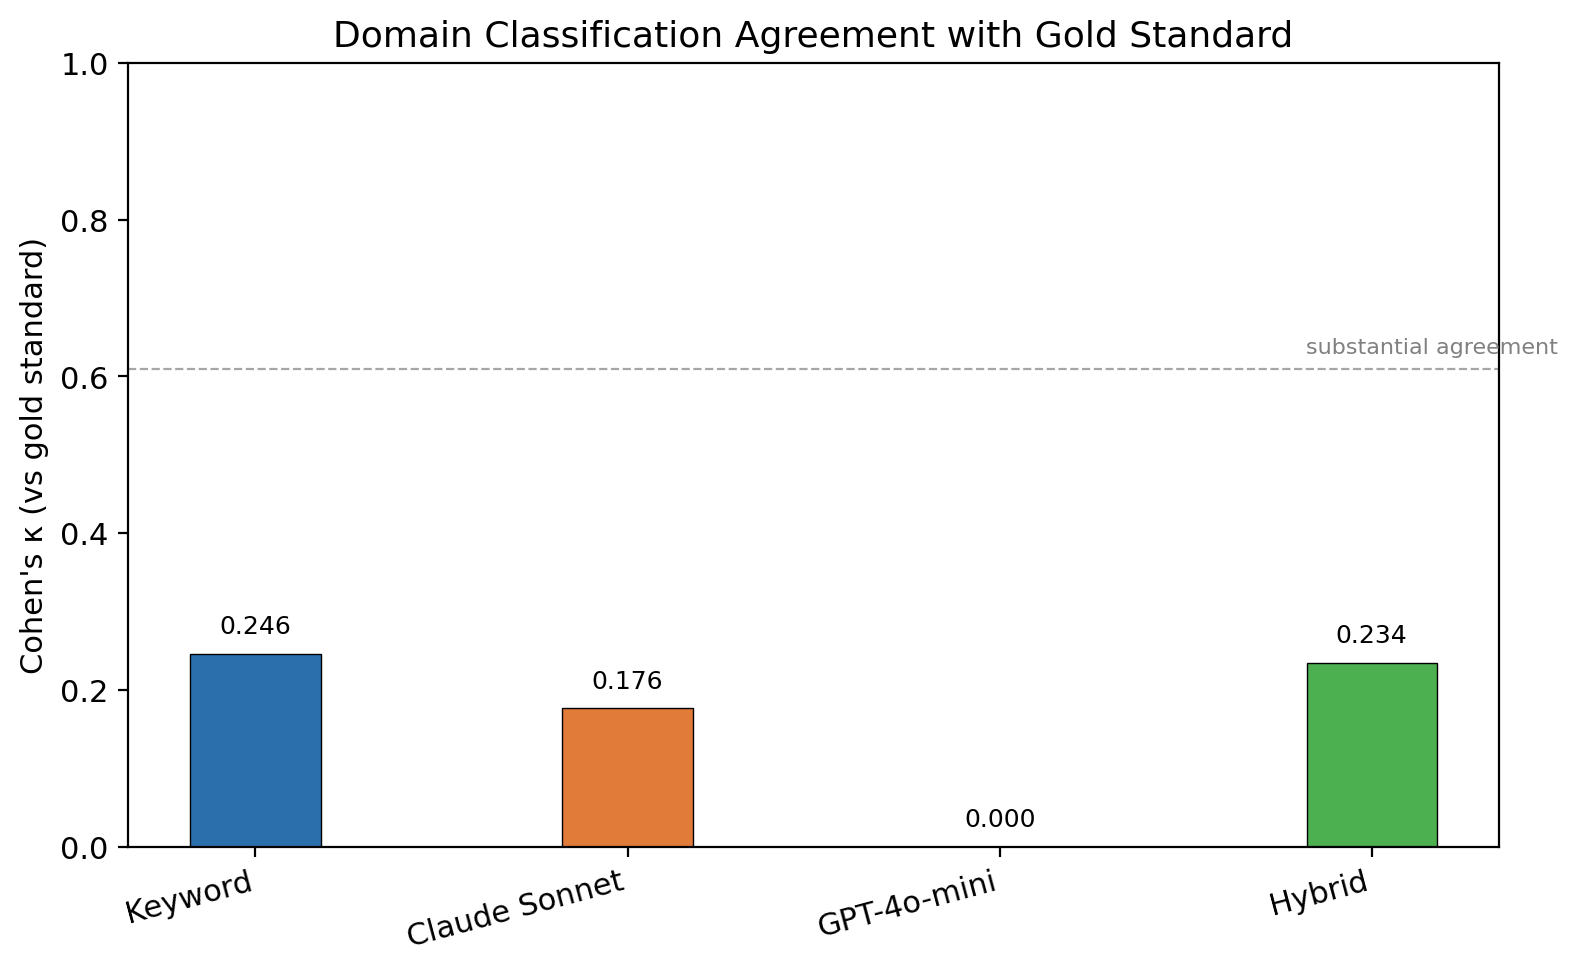
\includegraphics[width=0.85\textwidth]{figures/fig_multi_model_kappa.png}
\caption{Cohen's $\kappa$ agreement with gold standard across annotation methods}
\label{fig:multi-model-kappa}
\end{figure}

\begin{figure}[htbp]
\centering
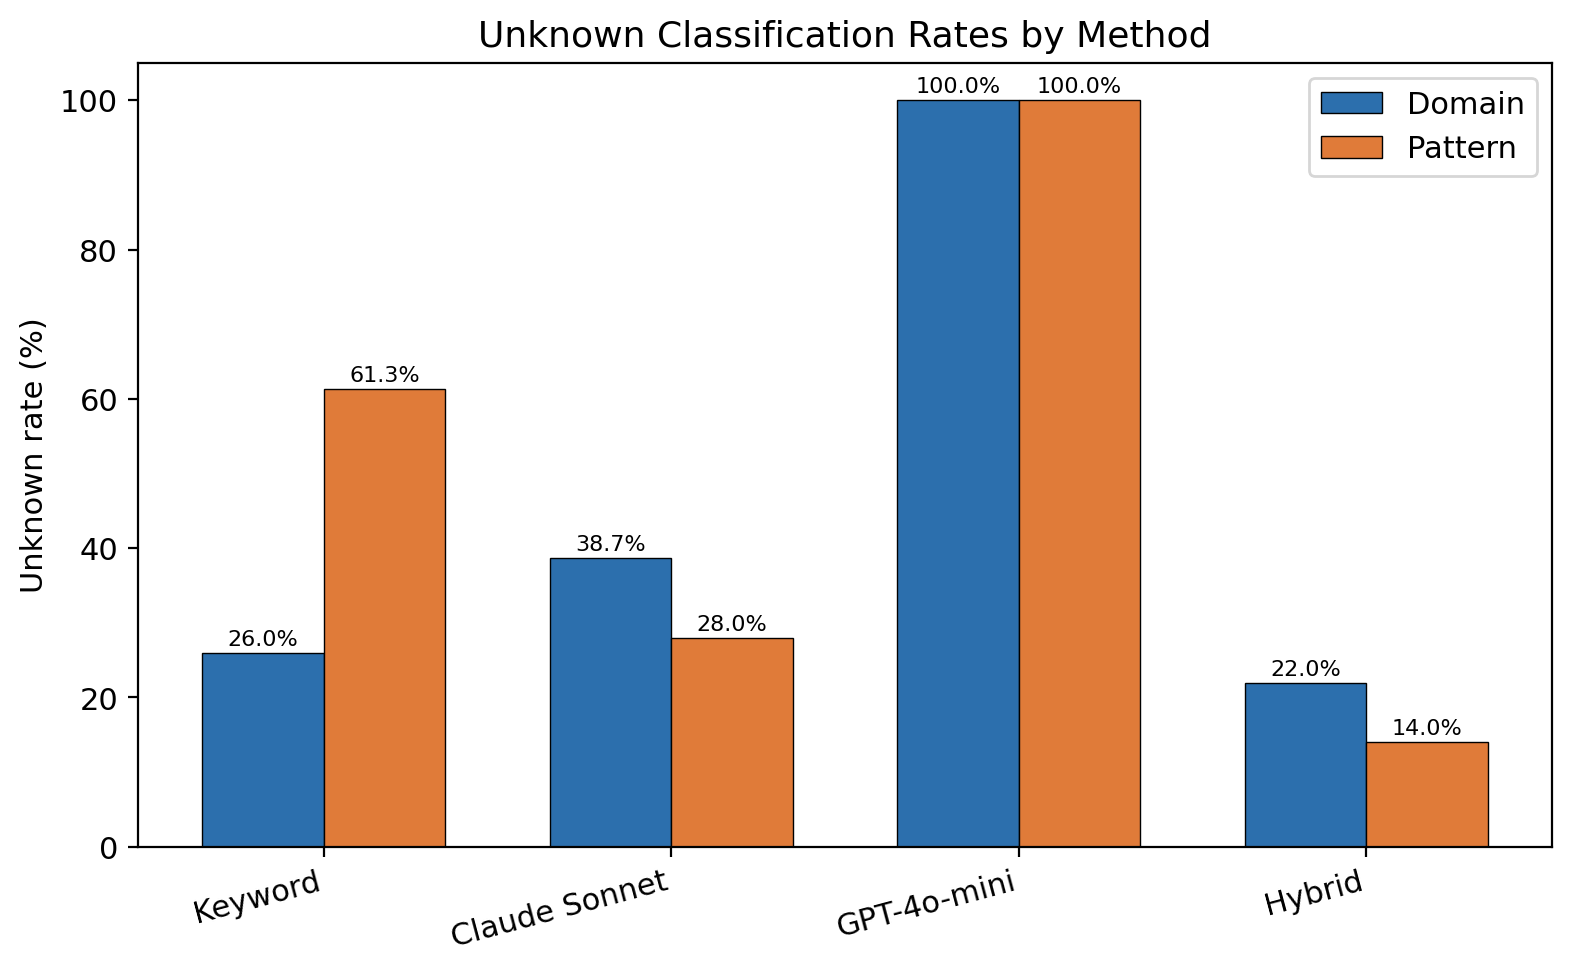
\includegraphics[width=0.85\textwidth]{figures/fig_multi_model_unknown_rates.png}
\caption{Unknown classification rates by method and axis}
\label{fig:multi-model-unknown}
\end{figure}

The results indicate that both LLMs produce broadly comparable domain classifications. GPT-4o-mini achieves a domain $\kappa$ of 0.000 against the gold standard, compared to Claude Sonnet's 0.176. The inter-model agreement ($\kappa = 0.000$) suggests that both models interpret the classification schema in a consistent manner, lending support to the hypothesis that the annotation framework is robust to the choice of underlying LLM.

The unknown rates for GPT-4o-mini on the domain axis (100.0%) and pattern axis (100.0%) are comparable to those observed for Claude Sonnet, indicating that classification uncertainty is driven primarily by the inherent ambiguity of the task rather than model-specific limitations. In particular, employment-domain classification remains challenging for both models, consistent with the observation that Annex~III(4) boundaries are less clearly delineated in incident descriptions than those of Annex~III(5a).

These findings strengthen the external validity of the framework. The consistency across two distinct model families --- Anthropic Claude and OpenAI GPT --- suggests that the classification schema captures genuine semantic distinctions in the incident data, rather than artefacts of a particular model's training distribution. This is a necessary (though not sufficient) condition for the framework's adoption as a reusable FRIA evidence-gathering tool.
